%%%%%%%%%%%%%%%%%%%%%%%%%%%%%%%%%%%%%%%%%
% Masters/Doctoral Thesis 
% LaTeX Template
% Version 1.43 (17/5/14)
%
% This template has been downloaded from:
% http://www.LaTeXTemplates.com
%
% Original authors:
% Steven Gunn 
% http://users.ecs.soton.ac.uk/srg/softwaretools/document/templates/
% and
% Sunil Patel
% http://www.sunilpatel.co.uk/thesis-template/
%
% License:
% CC BY-NC-SA 3.0 (http://creativecommons.org/licenses/by-nc-sa/3.0/)
%
% Note:
% Make sure to edit document variables in the Thesis.cls file
%
%%%%%%%%%%%%%%%%%%%%%%%%%%%%%%%%%%%%%%%%%

%----------------------------------------------------------------------------------------
%	PACKAGES AND OTHER DOCUMENT CONFIGURATIONS
%----------------------------------------------------------------------------------------

\documentclass[11pt, oneside]{Report} % The default font size and one-sided printing (no margin offsets)

\graphicspath{{Figures/}} % Specifies the directory where pictures are stored

\usepackage[square, numbers, comma, sort&compress]{natbib} % Use the natbib reference package - read up on this to edit the reference style; if you want text (e.g. Smith et al., 2012) for the in-text references (instead of numbers), remove 'numbers' 
\usepackage{adjustbox}
\hypersetup{urlcolor=blue, colorlinks=true} % Colors hyperlinks in blue - change to black if annoying
\title{\ttitle} % Defines the thesis title - don't touch this
\usepackage{float}
\usepackage{algorithm}
\usepackage{algpseudocode}
\usepackage{tikz}
\begin{document}

\newcommand\hlight[1]{\tikz[overlay, remember picture,baseline=-\the\dimexpr\fontdimen22\textfont2\relax]\node[rectangle,fill=blue!50,rounded corners,fill opacity = 0.2,draw,thick,text opacity =1] {$#1$};}


\frontmatter % Use roman page numbering style (i, ii, iii, iv...) for the pre-content pages

\setstretch{1.3} % Line spacing of 1.3

% Define the page headers using the FancyHdr package and set up for one-sided printing
\fancyhead{} % Clears all page headers and footers
\rhead{\thepage} % Sets the right side header to show the page number
\lhead{} % Clears the left side page header

\pagestyle{fancy} % Finally, use the "fancy" page style to implement the FancyHdr headers

\newcommand{\HRule}{\rule{\linewidth}{0.5mm}} % New command to make the lines in the title page

% PDF meta-data
\hypersetup{pdftitle={\ttitle}}
\hypersetup{pdfsubject=\subjectname}
\hypersetup{pdfauthor=\authornames}
\hypersetup{pdfkeywords=\keywordnames}

\makeatletter
\def\@makechapterhead#1{%
  \vspace*{50\p@}%
  {\parindent \z@ \raggedright \normalfont
    \ifnum \c@secnumdepth >\m@ne
      \if@mainmatter
        %\huge\bfseries \@chapapp\space \thechapter
        \Huge\bfseries \thechapter.\space%
        %\par\nobreak
        %\vskip 20\p@
      \fi
    \fi
    \interlinepenalty\@M
    \Huge \bfseries #1\par\nobreak
    \vskip 40\p@
  }}
\makeatother

%----------------------------------------------------------------------------------------
%	TITLE PAGE
%----------------------------------------------------------------------------------------

\begin{titlepage}
\begin{center}
	\begin{minipage}[t]{0.48\textwidth}
	  \begin{flushleft}
	  	    
\includegraphics [width=30mm]{Figures/logo} 
	  \end{flushleft}
	\end{minipage}
	\begin{minipage}[t]{0.48\textwidth}
	  \begin{flushright}
	  \end{flushright}
	\end{minipage} \\[2cm]
	
\textsc{\Large \subjectname}\\[0.3cm] % Thesis type

\HRule \\[0.4cm] % Horizontal line
{\huge \bfseries \ttitle}\\[0.4cm] % Thesis title
\HRule \\[1.5cm] % Horizontal line
 %\includegraphics [scale=0.55]{Figures/optimod} \\[1.5cm]
\begin{minipage}[t]{0.5\textwidth}
\begin{flushleft} \large
\emph{Author}\\
{\authornames}
\end{flushleft}
\end{minipage}
\begin{minipage}[t]{0.4\textwidth}
\begin{flushright} \large
\emph{Professor} \\
{\supname}
\end{flushright}
\end{minipage}\\[0.7cm]

\vfill
\footnotesize{\today}


\end{center}

\end{titlepage}



%----------------------------------------------------------------------------------------
%	LIST OF CONTENTS/FIGURES/TABLES PAGES
%----------------------------------------------------------------------------------------

\pagestyle{fancy} % The page style headers have been "empty" all this time, now use the "fancy" headers as defined before to bring them back

%\lhead{\emph{Contents}} % Set the left side page header to "Contents"
%\tableofcontents % Write out the Table of Contents

%\lhead{\emph{Figures}} % Set the left side page header to "List of Figures"
%\listoffigures % Write out the List of Figures

%\lhead{\emph{Tables}} % Set the left side page header to "List of Tables"
%\listoftables % Write out the List of Tables


%----------------------------------------------------------------------------------------
%	CONTENT - CHAPTERS
%----------------------------------------------------------------------------------------
\mainmatter % Begin numeric (1,2,3...) page numbering

\pagestyle{fancy} % Return the page headers back to the "fancy" style
% Chapter Template

\chapter{Introduction} % Main chapter title

\label{Intoduction} % Change X to a consecutive number; for referencing this chapter elsewhere, use \ref{ChapterX}

\lhead{1. \emph{Introduction}} % Change X to a consecutive number; this is for the header on each page - perhaps a shortened title

%----------------------------------------------------------------------------------------
%	SECTION 1
%----------------------------------------------------------------------------------------

The magic word model generates $N$ sequences of length $M$, $s^1,\dots,s^N$, where $s^n = s_1^n,\dots, s_M^n$, where all the sequences are over an alphabet $[K].$ Each sequence has a magic word of length $W$ hidden in it, while the rest of the sequence is called background. Our goal is to find $R=r_1, \dots,r_N$, where $r_n$ is the start position of the magic word in the $n$:th sequence $s^n$.

An interesting application of this model can be found in biosequence analysis. The alphabet that we consider is the genomic alphabet: $K = \{ A, C, G, T\}$. The sequences $s^1,\dots,s^N$ become a set of aligned DNA sequences and the positions $[1\dots M]$ are the DNA columns which represent locations along the genome. Our problem can therefore be  reformulated as finding the unknown magic word that appears at different unknown starting positions in those sequences. 

In order to do that, we will implement a collapsed Gibbs sampler to sample from the posterior $p(r_1, \dots, r_N|D)$ where D is the set of DNA sequences generated by the model.

% Chapter Template
\chapter{Generation} % Main chapter title

\label{Generation} % Change X to a consecutive number; for referencing this chapter elsewhere, use \ref{ChapterX}

\lhead{2. \emph{Generation}} % Change X to a consecutive number; this is for the header on each page - perhaps a shortened title

%----------------------------------------------------------------------------------------
%	SECTION 1
%----------------------------------------------------------------------------------------

The magic word generative model proceeds as follow:

\begin{itemize}
\item For each sequence $s^n$ in $s^1 \dots s^N$, we sample a start position $r_n \sim U(M-W+1)$
\item Then for each sequence, we sample the letters in the positions $j$ in the magic word : 
\begin{equation*}
x^n_j \sim Cat(\theta_j) 
\end{equation*}
Where $\theta_j \sim Dir(\alpha)$ and $j \in [r_n, r_n + W - 1]$
\item Finally, we sample the letters in the background positions for all sequences:
\begin{equation*}
x^n \sim Cat(\theta) \quad \text{Where} \quad \theta \sim Dir(\alpha')
\end{equation*}
\end{itemize}
Since we have no prior specific knowledge about the background of the DNA sequences, we will use a uniform prior for $\theta$ with parameter $\alpha' = \begin{pmatrix}
1&1&1&1
\end{pmatrix}$. All sequences will be generated from the same categorical distribution. For the magic words in the sequences however, the $j$:th positions are generated from distinct categorical distributions parameters $\theta_j$ having the same prior $Dir(\alpha)$, which complicates accurate inference. 
We generate set of 5 sequences ($N=5$) and 30 columns ($M=10$), with magic words of length 10 ($W= 5 $), with $\alpha' = (1, 1,1,1)$ and $\alpha = (12,7,3,1)$. The start positions are highlighted:
\begin{equation*}
\begin{matrix}
A & T & T & A & \hlight{C} & G & C & A & A & T \\
T & A & T & T & \hlight{A} & A & C & G & A & C \\
\hlight{C} & G & C & C & A & C & A & C & C & A \\
C & G & C & T & A & \hlight{A} & A & G & A & A \\
A & T & A & A & T & \hlight{A} & G & A & G & A 
\end{matrix}
\end{equation*}
% Chapter Template

\chapter{Gibbs Sampler} % Main chapter title

\label{Gibbs} % Change X to a consecutive number; for referencing this chapter elsewhere, use \ref{ChapterX}

\lhead{3. \emph{Gibbs Sampler}} % Change X to a consecutive number; this is for the header on each page - perhaps a shortened title

%----------------------------------------------------------------------------------------
%	SECTION 1
%----------------------------------------------------------------------------------------
We use a Gibbs sampler to estimate the posterior $p(r_1, \dots, r_N | D)$ where $D$ is the set of sequences $s^1, \dots, s^N$ generated by the magic word model and $r_n$ is the start position of the magic word in the $n$:th sequence $s^n$.

We use a \textit{collapsed} Gibbs sampler, which means collapse out the Dirichlet distributions(the prior distributions over the categorical variables). The result of this collapsing introduces dependencies among all the categorical variables dependent on a given Dirichlet prior.

Each state $R^{(s)}$ of a the Markov chain has the following form : $R^{(s)} = r_1^{(s)} \dots r_N^{(s)}$.

The first $T$ samples (burn-in period) are discarded to allow for the Markov chain to reach stationarity. We also collect subsequent samples after a lag to ensure their correlation is low.

The implementation is as follows: 

\begin{algorithmic}[1]
\State Random initialization $R^{(0)}$
\For{i from 0 to iterations}
    \For{n from 0 to N}
            \State $P(r^{(i)}_{n}|R_{-n}^{(i)}, D) \propto \cup_{l = 0}^{M-W-1} p(D_{background}| R^{(i)},\alpha') \prod\limits_{j = l}^{l + W} p(D_{j}|R^{(i)},\alpha)$
            \State normalize the above vector of probabilities
        \State $r^{(i)}_{n} \sim Cat(P(r^{(i)}_{n}|R_{-n}^{(i)}, D))$ \Comment $r^{(i)}_{n}$ is sampled from the categorical with parameter $P(r^{(i)}_{n}|R_{-n}^{(i)}, D)$, which is the vector of posterior probabilities for values of $r^{(i)}_{n}$ in $[0, M-W-1]$
    \EndFor
\EndFor

\For{n from 0 to N}
    \State samples = samples[i] \Comment samples is the vector containing the Markov chain states (samples) that were collected
    \State $r_n = argmax(count_{t = T:k:iterations}(R^{(t)}_{n}))$ \Comment For each sequence, the starting position is the mode of the posterior, i.e. the position that was sampled most frequently . The $T$ first samples are discarded and we only consider every $k$:th iteration in the samples, where $k > 1$.
\EndFor
\end{algorithmic}

With : 

\begin{equation}
p(D_{background}|R^{(i)}, \alpha') = \frac{\Gamma(\sum_k \alpha'_k)}{\Gamma(B \sum_k \alpha'_k)} \prod_k \frac{\Gamma(B_k + \alpha'_k)}{\Gamma(\alpha'_k)}
\end{equation}
where $B = N(M-W))$ is the number of background positions and $B_k$ is the count of symbol $k$ in the background.
\begin{equation}
p(D_{j}|R^{(i)},\alpha) = \frac{\Gamma(\sum_k \alpha_k)}{\Gamma(N \sum_k \alpha_k)} \prod_k \frac{\Gamma(N^j_k + \alpha_k)}{\Gamma(\alpha_k)}
\end{equation}
where $N^j_k$ is the count of symbol $k$ in the $j$:th column of the magic word.

% Chapter Template

\chapter{Results} % Main chapter title

\label{Results} % Change X to a consecutive number; for referencing this chapter elsewhere, use \ref{ChapterX}

\lhead{4. \emph{Results}} % Change X to a consecutive number; this is for the header on each page - perhaps a shortened title

%----------------------------------------------------------------------------------------
%	SECTION 1
%----------------------------------------------------------------------------------------
 We consider a model with 5 sequences ($N=5$) and 30 columns ($M=30$), with magic words of length 10 ($W= 10 $). 
 
 \section{Convergence}
 We first want to estimate the number of iterations that are necessary for the Markov chain to converge to the target distribution. We run the sampler for 200 iterations, with $\alpha' = (1, 1,1,1)$ and $\alpha = (12,7,3,1)$ and obtain the results in figure \ref{fig:1}. We can see that the burn-in period is almost undetectable and the chain converges rapidly. Nonetheless, to estimate the accuracy, we discard the first $100$ samples and save the subsequent samples with a lag of $10$. We obtain an accuracy of $80\%$ : the true starting positions being $[11, 11, 18, 5, 4]$ and the estimated positions being $[11, 12, 18, 5, 4]$. We can also note that for the second sequence, the estimated start position 12 is close to the true start position 11, and inside the magic word.
 \begin{figure}[htbp]
  \centering
    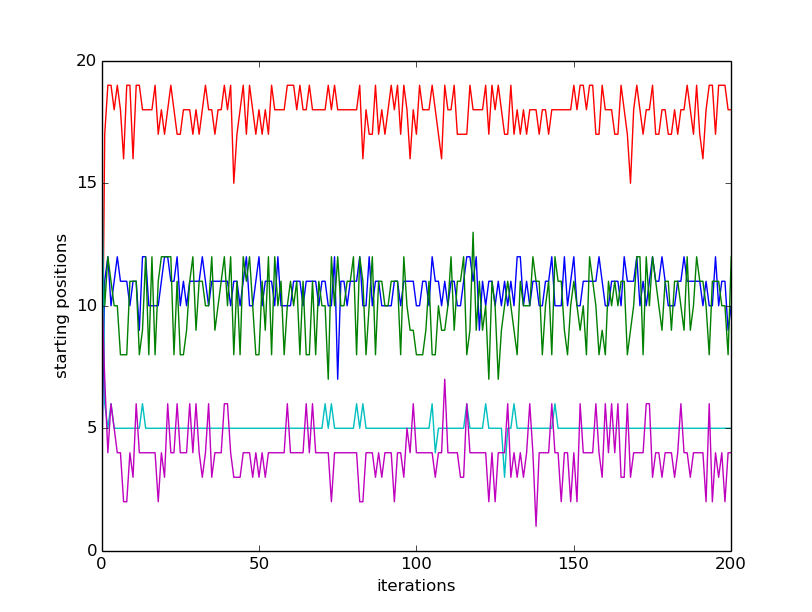
\includegraphics[scale = 0.75]{Figures/fig1}
  \caption{Markov chain samples for $\alpha' = (1, 1,1,1)$ and $\alpha = (12,7,3,1)$}
  \label{fig:1}
\end{figure}

Another way to check the convergence of the Markov Chain is to estimate how far the samples are from perfect mixing. We can therefore compute the R.hat (potential scale reduction factor). For that, we run 3 chains, compute the variance of the samples from each chain (after the halves of each have been discarded. We also compute the variance of all the chains mixed together. 
\begin{equation*}
R.hat = \sqrt{\frac{\text{mixture variance}}{\text{average within the chain variances}}}
\end{equation*}
After 200 iterations of the chain described above, we obtain : $R.hat = 1.02$, which indicates that the chain has converged, since the distributions between and within the chains are identical.

\section{Effect of $\alpha$}

The accuracy of the estimation depends on whether the categorical distributions of the magic words and of the background are distinguishable. It would therefore follow that the more skewed $\alpha$ is, or the more different from $\alpha'$, the higher the accuracy will be.

Since the accuracy can be highly dependent on the sequences we generated, we compute the average accuracy for $500$ sets of sequences, for different vectors $\alpha$. The results are presented in table \ref{alpha}

\begin{table}[h]
\centering
\caption{Accuracy for different values of $\alpha$. model with $\alpha' = (1, 1,1,1)$}
\label{alpha}
\begin{tabular}{|l|l|}
\hline
$\alpha$              & Accuracy \\ \hline
$(12, 7, 3, 1)$       & 0.61        \\ \hline
$(12, 7, 20, 16)$     & 0.63       \\ \hline
$(2, 2, 2, 2)$        & 0.402       \\ \hline
$(12, 1, 1, 1)$ & 0.74       \\ \hline
\end{tabular}
\end{table}

The lowest accuracy is for $\alpha = (2, 2, 2, 2)$ as expected, since it is very close to the prior for the background. Wee can see the accuracy the highest when the Dirichlet parameter is “tilted” towards one of the letters $\alpha = (12, 1, 1, 1)$. The difference between the components of $\alpha$ and $alpha'$ seems to have less impact on the accuracy than the skewness of $Dir(\alpha)$.
Figure \ref{fig:2} shows the convergence plot for a set of sequences using $\alpha' = (1, 1,1,1)$ and $\alpha = (12, 1, 1, 1)$. The accuracy for this data set is $80\%$: the true positions are $[1,9,17,5,11]$ and the estimated positions are $[1,9,17,5, 10]$.  

 \begin{figure}[htbp]
  \centering
    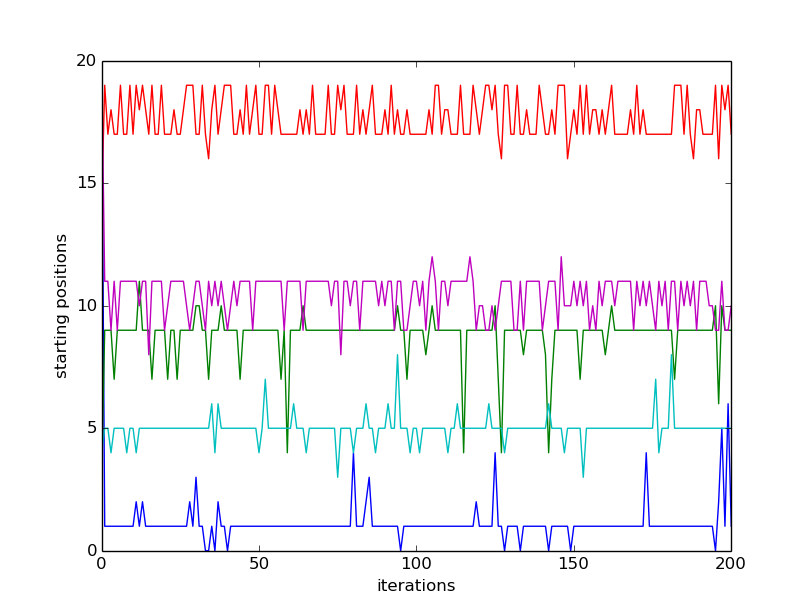
\includegraphics[scale = 0.75]{Figures/fig2}
  \caption{Markov chain samples for $\alpha' = (1, 1,1,1)$ and $\alpha = (12, 1, 1, 1)$}
  \label{fig:2}
\end{figure}

\section{Effect of the lag}
We have considered that the estimated starting position is the mode of the posterior distribution $p(r_n | R_{-n}, D)$. It seems reasonable to think that the less correlated the samples we draw (after convergence) are, the more accurate our estimation of the node will be. To verify this, we compute the average accuracy for $500$ sets of sequences, for different values of the lag. To get a better estimation of the mode, we run the Gibbs sampler for $500$ iterations but only discard the first $100$ samples, since we have seen that the convergence is achieved rapidly. The results are presented in table \ref{lag}

\begin{table}[h]
\centering
\caption{Accuracy for different lag lengths, model with $\alpha' = (1, 1,1,1)$ and $\alpha = (12,7,3,1)$}
\label{lag}
\begin{tabular}{|l|l|}
\hline
Lag        & Accuracy \\ \hline
1 (no lag) &     0.66    \\ \hline
10 samples &     0.67    \\ \hline
30 samples &     0.63    \\ \hline
\end{tabular}
\end{table}
 
As we can see, the difference between no lag and a lag of 10 samples is not significant, and with a lag of 30 samples, the average accuracy is even slightly lower. we conclude that the purpose of saving every $k$th iteration for our application is not statistical, since the correlation doesn't seem to influence the accuracy. However, it could have computational benefits if we run multiple chains with a very high number of samples in parallel and do not want to carry them all around in our simulation.
 

%----------------------------------------------------------------------------------------
%	THESIS CONTENT - APPENDICES
%----------------------------------------------------------------------------------------

\addtocontents{toc}{\vspace{2em}} % Add a gap in the Contents, for aesthetics

%\appendix % Cue to tell LaTeX that the following 'chapters' are Appendices

% Include the appendices of the thesis as separate files from the Appendices folder
% Uncomment the lines as you write the Appendices

%\input{Appendices/AppendixA}
%\input{Appendices/AppendixB}
%\input{Appendices/AppendixC}

\addtocontents{toc}{\vspace{2em}} % Add a gap in the Contents, for aesthetics

\backmatter

\end{document}